% ----------------------------------------------------------
% Subseção Consciência
% ----------------------------------------------------------
\subsection{Consciência}
Um momento lógico pode ser formado por uma divisão (primeiro momento) ou por subdivisões lógicas (demais momentos).
	\begin{figure}[H]
	\caption{Intervalo lógico}
	\label{fig:consciousness_logical_moments}
	\centering
	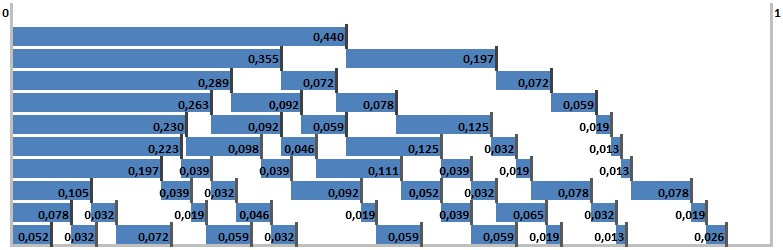
\includegraphics[scale=.7]{sections/images/consciousness_logical_moments.jpg}
	\floatfoot{Exemplo de um intervalo lógico com dez momentos lógicos.}%\footnotemark}
	\end{figure}
	%\footnotetext{Fonte: note}

A consciência são os momentos lógicos de uma expansão representados em suas unidades.
	\begin{figure}[H]
	\caption{Intervalo lógico consciente}
	\label{fig:consciousness}
	\centering
	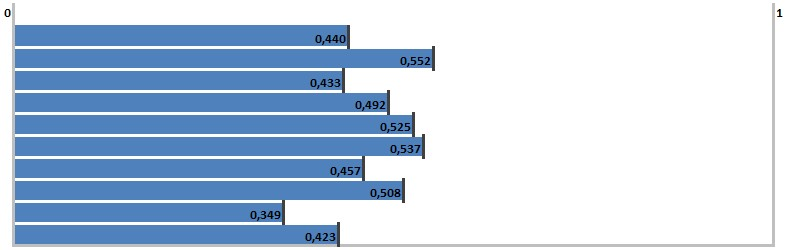
\includegraphics[scale=.7]{sections/images/consciousness.jpg}
	\floatfoot{Exemplo de um intervalo lógico consciente com dez unidades de momentos lógicos.}%\footnotemark}
	\end{figure}
	%\footnotetext{Fonte: note}

Pode ser observado na Tabela \ref{tab:10000_all} que a probabilidade de 99,99\% das amostras de uma população (Amostras do Range), que aumentam em quantidade à medida que crescem os momentos lógicos, tendem a estar cada vez mais ao centro do intervalo lógico, sendo que essa centralização tende ao infinito.
	\begin{figure}[H]
	\caption{Centralização de 99,99\% das amostras}
	\label{fig:centering_of_99_range}
	\centering
	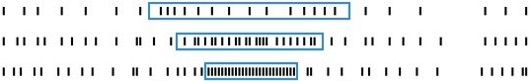
\includegraphics[scale=1]{sections/images/centering_of_99_range.jpg}
	\floatfoot{Tendência de centralização do range de 99,99\% das amostras.}%\footnotemark}
	\end{figure}
	%\footnotetext{Fonte: note}

A consciência tende à representação de uma onda lógica, a maior onda lógica de uma população, um histograma da distribuição normal. Todos os aspectos listados abaixo são inerentes a abstração lógica chamada consciência.

\subsubsection{Infinito}
Um dos aspectos mais importantes que a negação do nada traz (negação de si), é o infinito, ou seja, em qualquer intervalo lógico cabe o infinito novamente. A lógica primordial que iniciou todo o intervalo lógico é a mesma encontrada em seus intervalos subsequentes. Isso fundamenta como uma lógica de alto nível como a subconsciência humana explica a lógica primordial, uma vez que não é preciso voltar ao primeiro momento lógico do intervalo para deduzi-lo, pois esse fenômeno é onipresente em todo o intervalo.

\subsubsection{Ondas}
Probabilisticamente a distribuição de novas amostras de uma população tendem a concentrar mais amostras sentido a mediana da população com frequências de amostras cada vez maiores neste sentido. Porém, a distribuição dessas amostras com frequências de crescimento uniformes é infinitesimal se comparado às possibilidades randômicas desse crescimento. Assim, a tendência de crescimento dessas frequências sentido a mediana somadas a baixíssima probabilidade (infinitesimal) desse crescimento ser uniforme, conduz a frequências no padrão de ondas. A relação de densidade ou amplitude de uma onda com seu comprimento é detalhada nas subseções do Espaço, Comprimento de onda e Amplitude de onda.
	\begin{figure}[H]
	\caption{Padrão de onda}
	\label{fig:consciousness_waves}
	\centering
	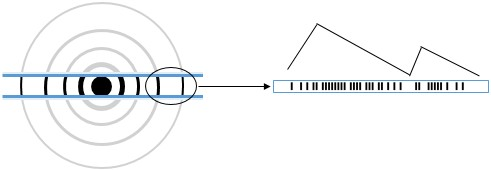
\includegraphics[scale=1]{sections/images/consciousness_waves.jpg}
	\floatfoot{Padrão de onda inferido pela tendência dessa distribuição com frequências maiores sentido a mediana da população e a baixíssima probabilidade de crescimento uniforme dessas frequências.}%\footnotemark}
	\end{figure}
	%\footnotetext{Fonte: note}

A junção de duas ondas além de eliminar suas discrepâncias, faz com que a primeira onda da união fique maior e a segunda onda acabe por deixar de existir a se tornar parte da primeira, que tem seu pico mais próximo da mediana. Probabilisticamente uma onda não morre, apenas une-se com outras ondas mais centrais a ela.
	\begin{figure}[H]
	\caption{Unificação de ondas}
	\label{fig:consciousness_uniform_wave}
	\centering
	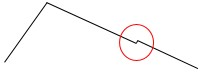
\includegraphics[scale=1]{sections/images/consciousness_uniform_wave.jpg}
	\floatfoot{Ondas sendo unificadas para exemplificar o crescimento amostral uniforme.}%\footnotemark}
	\end{figure}
	%\footnotetext{Fonte: note}

\subsubsubsection{Comprimento e amplitude}
O histograma é utilizado nas figuras dessa subseção e posteriormente para facilitar a visualização e entendimento, pois representa muito bem a curva de densidade de uma população, conforme as diferentes visualizações da Figura \ref{fig:consciousness_wave_histogram} representando apenas um intervalo ou um comprimento de onda pareado pela mediana da população.  
	\begin{figure}[H]
	\caption{Histograma em diferentes visualizações }
	\label{fig:consciousness_wave_histogram}
	\centering
	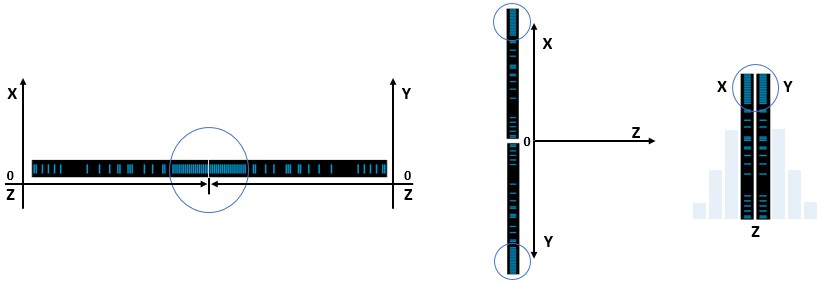
\includegraphics[scale=.7]{sections/images/consciousness_wave_histogram.jpg}
	\floatfoot{Diferentes maneiras da representação populacional em histograma.}%\footnotemark}
	\end{figure}
	%\footnotetext{Fonte: note}}
O comprimento e amplitude de ondas estabelecem uma relação de quantidade por intervalo ou unidade. Essas unidades são estabelecidas pelo entrelaçamento de ondas, conforme subseção posterior. Assim, a amplitude é a densidade de um comprimento de onda, a densidade de um intervalo qualquer.  

Ao adicionar uma nova amostra na população todo o intervalo se distribui proporcionalmente para acoplar essa amostra. Ao observar a população em intervalo ou comprimentos de ondas menores suas amplitudes de ondas obedecerão a distribuição de amostras desses subintervalos proporcionalmente, conforme Figura \ref{fig:consciousness_space_volume_amplitude}.
	\begin{figure}[H]
	\caption{Comprimento vs Amplitude de onda}
	\label{fig:consciousness_space_volume_amplitude}
	\centering
	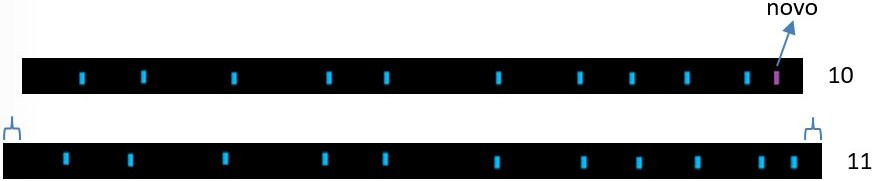
\includegraphics[scale=.4]{sections/images/consciousness_space_volume_amplitude.jpg}
	\floatfoot{Relação de comprimento e amplitude de ondas.}%\footnotemark}
	\end{figure}
	%\footnotetext{Fonte: note}}

Outro fator importante é que ao adicionar uma nova amostra em uma coluna, como na coluna azul da Figura \ref{fig:consciousness_space_amplitude_growth}. Mesmo que no início da coluna, essa nova amostra fará com que está coluna cresça proporcionalmente à adição dessa nova amostra e somente o subconjunto 4 terá o crescimento proporcional total dessa coluna. Assim a adição de uma amostra nessa coluna no subconjunto 0, faria o subconjunto 0 alongar 1/5 de uma amostra nessa coluna, o subconjunto 1 alongar 2/5 de uma amostra até o subconjunto 4 alongar 5/5 de uma amostra nessa coluna. Isso somada à maior distribuição de amostras no pico da coluna podem facilitar o entendimento do adiantamento dos relógios atómicos nos satélites.
	\begin{figure}[H]
	\caption{Amplitude de onda - crescimento proporcional}
	\label{fig:consciousness_space_amplitude_growth}
	\centering
	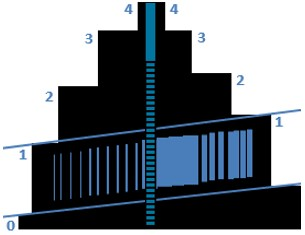
\includegraphics[scale=.7]{sections/images/consciousness_space_amplitude_growth.jpg}
	\floatfoot{Relação de proporção no crescimento da amplitude de ondas.}%\footnotemark}
	\end{figure}
	%\footnotetext{Fonte: note}}

Em grandes intervalos com muitos momentos lógicos é observado uma discrepância menor das amplitudes das ondas. Nesses intervalos podem ser observados grandes sistemas de objetos (subconsciências). Quanto maiores os agrupamentos mais largas e curtas são as ondas, proporcionalmente, conforme Figura \ref{fig:consciousness_space_subconsciousness}. A onda mais inferior, azul escuro, é a onda base do sistema, ou seja, a onda formadora de outras ondas. Os sistemas de ondas podem ser mais complexos, tendo várias ondas aninhadas. Intervalos mais complexos e com essa característica podem representar, por exemplo, o centro do universo, então o centro de uma galáxia, estrelas, planetas e objetos menores e mais distantes.
	\begin{figure}[H]
	\caption{Abstração espacial das subconsciências - grandes agrupamentos}
	\label{fig:consciousness_space_subconsciousness}
	\centering
	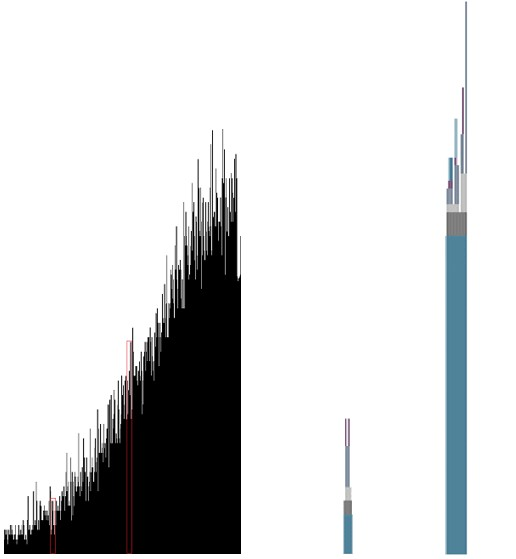
\includegraphics[scale=.45]{sections/images/consciousness_space_subconsciousness.jpg}
	\floatfoot{Caracteristicas da ondas formadoras da subconsciência de grandes objetos.}%\footnotemark}
	\end{figure}
	%\footnotetext{Fonte: note}

Em intervalos menores e com muitos momentos lógicos é observado uma discrepância maior das amplitudes das ondas. Nesses intervalos podem ser observados sistemas menores de objetos (subconsciências). Quanto menores os agrupamentos mais comprida e estreita são as ondas, proporcionalmente, conforme Figura \ref{fig:consciousness_space_subconsciousness_min}. A onda mais inferior, azul escuro, é a onda base do sistema, ou seja, a onda formadora de outras ondas. Os sistemas de ondas podem ser mais complexos, tendo várias ondas aninhadas. Intervalos mais complexos e com essa característica podem representar, por exemplo, o átomo que são muito pequenos, se apresentam em enormes quantidades e as partículas que orbitam seu núcleo (elétrons) ficam bem mais distantes dele.
	\begin{figure}[H]
	\caption{Abstração espacial das subconsciências - pequenos agrupamentos}
	\label{fig:consciousness_space_subconsciousness_min}
	\centering
	
\includegraphics[scale=.6]{sections/images/consciousness_space_subconsciousness_min.jpg}
	\floatfoot{Caracteristicas da ondas formadoras da subconsciência de pequenas partículas.}%\footnotemark}
	\end{figure}
	%\footnotetext{Fonte: note}}

\subsubsubsection{Entrelaçamento}
As amostras que mais se parecem em termos de frequências e distribuição são as amostras que fazem parte da mesma onda. Elas são frequências opostas não sobrepostas que se completam.

Probabilisticamente as duas partes complementares de uma onda estarão a uma distância aproximadamente iguais, equidistante da mediana, porém essa não é uma regra e as partes complementares de uma onda podem estar em distâncias diferentes da mediana. O fenômeno da paridade das partes de uma onda tem o nome de entrelaçamento de ondas.

Esses pares são formados pela probabilidade, onde comprimentos de ondas iguais detém a mesma probabilidade de distribuição de amostras em dois pontos diferentes da população. 

Essas ondas formam subconsciências de uma consciência maior, a maior de todas as ondas. A consciência é única para todo o intervalo, é a lógica do intervalo, enquanto formam subconsciências ou sub-lógicas, como pequenas ondas de uma onda maior e semelhantes ao padrão dessa onda maior. Assim, uma mudança na onda maior (consciência) também é uma mudança na onda menor (subconsciência), mudança essa que é induzida pelas subconsciências indiretamente, análogo ao comprimir gás em um cilindro, onde ao adicionar uma nova molécula de gás no cilindro parcialmente cheio mais próximas ou apertas as moléculas dentro dele estarão. O contrário também é verdadeiro, uma nova amostra em uma subconsciência que por esta é observada diretamente é também uma mudança da consciência e vai ser induzida por outras subconsciências indiretamente.
	\begin{figure}[H]
	\caption{Subconsciência}
	\label{fig:consciousness_subconscious}
	\centering
	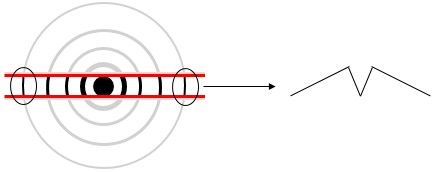
\includegraphics[scale=.8]{sections/images/consciousness_subconscious.jpg}
	\floatfoot{O padrão de ondas forma subconsciências semelhantes ao padrão criado pela consciência, como visto na Figura \ref{fig:statisticsbyjim_central_limit_theorem} ou na Figura \ref{fig:trend_chart_of_normal_distribution}.}%\footnotemark}
	\end{figure}
	%\footnotetext{Fonte: note}
	
O entrelaçamento de ondas pode ocorrer em diferentes níveis ou intervalos, conforme visto na Figura \ref{fig:consciousness_subconscious_entanglement}, o que forma sistemas. Os colchetes com bordas identificam os intervalos os quais uma nova amostra despertou o salto, conforme visto na próxima subseção, e os retângulos com bordas representam o intervalo que sofreu a reordenação. Os colchetes e retângulos sem bordas representam o par da onda na reordenação. Os arcos numerados indicam a ordem dos saltos.

O maior entrelaçamento é mostrado nos exemplo da Figura \ref{fig:consciousness_subconscious_entanglement} como o primeiro salto, que é mantido ordenado pelas reordenações dos subintervalos subsequentemente. Essa onda é comumente entrelaçada pela mediana da população e seu entrelaçamento talvez não seja exclusividade do primeiro salto. Os intervalos menores sofrem o entrelaçamento primeiro e essa reordenação causada por eles permite o entrelaçamento de pares com intervalos maiores. Os pares entrelaçados têm linhas de referências opostas, pois são os dois lados de uma onda (pico ou vale) e se entrelaçam por sua mediana, que pode coincidir com a mediana da população quando se trata da maior onda probabilística. 
	\begin{figure}[H]
	\caption{Níveis do entrelaçamento de ondas}
	\label{fig:consciousness_subconscious_entanglement}
	\centering
	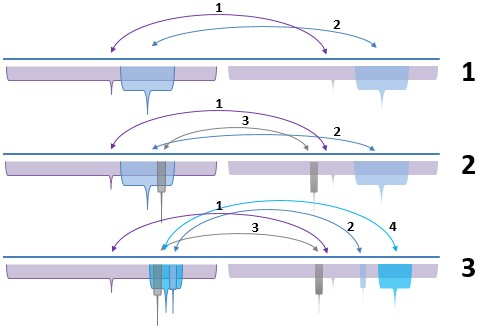
\includegraphics[scale=.9]{sections/images/consciousness_subconscious_entanglement.jpg}
	\floatfoot{Exemplos dos níveis do entrelaçamento de ondas.}%\footnotemark}
	\end{figure}
	%\footnotetext{Fonte: note}

Os exemplos da Figura \ref{fig:consciousness_subconscious_entanglement} mostram os subintervalos, picos ou vales, entrelaçados mais fortemente com outros intervalos não equidistantes. Os entrelaçamentos estão intimamente ligados aos comprimentos de ondas de uma população. Os possíveis comprimentos de ondas de uma população são definidos por esses níveis de entrelaçamentos de ondas.

O salto é uma reordenação feita pelo entrelaçamento de ondas para manter os pares equivalentes e essa reordenação ocorre apenas nos níveis do entrelaçamento, não alterando a ordem das amostras da população. Dessa forma, um intervalo entrelaçado tende a voltar para níveis de entrelaçamento inferiores à medida que a probabilidade de amostras desse intervalo transite temporariamente entre vale e pico ao equilíbrio. 

\subsubsubsection{Salto}
O salto é uma reordenação feita pelo entrelaçamento de ondas à medida em que as amostras dos pares entrelaçados deixam de ser equivalentes com a adição de novas amostras em seus pares. O salto ocorre em uma das partes do par de uma onda e é uma reordenação, ou seja, tanto a parte da onda A deve melhor se adequar a parte da onda B quanto o contrário. 

Na Figura \ref{fig:consciousness_space_subconscious_observation_jump} é observado os entrelaçamento de ondas (representadas por colunas de um histograma para facilitar a visualização do intervalo). A reordenação feita pelo entrelaçamento provoca um salto nas coordenadas (X, Y e Z) conforme subseção do Espaço.
	\begin{figure}[H]
	\caption{Reordenação - Salto}
	\label{fig:consciousness_space_subconscious_observation_jump}
	\centering
	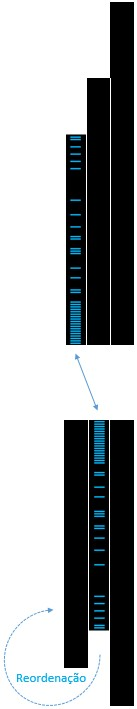
\includegraphics[scale=.55]{sections/images/consciousness_space_subconscious_observation_jump.jpg}
	\floatfoot{Salto provocado pela não equivalência do par entrelaçado com a adição de novas em um de seus lados.}%\footnotemark}
	\end{figure}
	%\footnotetext{Fonte: note}

A reordenação de um salto ocorre apenas nos níveis do entrelaçamento, não alterando a ordem das amostras da população. Um intervalo entrelaçado tende a transitar entre os níveis de entrelaçamento à medida que a probabilidade de amostras desse intervalo transitar temporariamente entre vale e pico ao equilíbrio. Assim, a tendência probabilística é que, por exemplo, o elétron que saltou de sua orbita de origem retorne à esta conforme mais amostras são adicionadas ao intervalo populacional desse átomo, reestabelecendo sua característica probabilística.

\subsubsection{Tempo}
O tempo é a adição de novos momento lógicos entre momentos existentes à medida que prossegue a negação de si da lógica. Essas mudanças são acumulativas e a medida que aumentam o número desses momentos lógicos, menos relevante cada novo momento será dentro do intervalo consciente. Um em cem é mais relevante do que um em mil. 
	\begin{figure}[H]
	\caption{Tempo}
	\label{fig:consciousness_time}
	\centering
	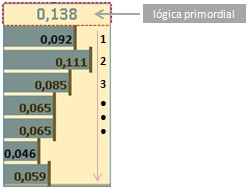
\includegraphics[scale=.8]{sections/images/consciousness_time.jpg}
	\floatfoot{Progressão do tempo conforme os momentos lógicos avançam.}%\footnotemark}
	\end{figure}
	%\footnotetext{Fonte: note}

Outro fator importante a observar do tempo é que, probabilisticamente, subconsciências mais próximas da mediana da população terão uma adição maior de novas amostras em seus intervalos, o que são observados diretamente por essas subconsciências. Por outro lado, subconsciências distantes da mediana da população terão uma adição menor de amostras em seus intervalos e sujeitam-se a um número maior de mudança induzidas indiretamente. Esse fenômeno de observação temporal proporcionado pela consciência e subconsciências evita o paradoxo dos gêmeos \cite{brasilescola_paradoxo_gemeos}.

Na seção Expansão lógica foi apresentado que a lógica é uma sequência de negações de si no tempo zero, ou seja, em nenhum momento entre suas negações a lógica passa a SER, garantindo a premissa primordial da constante lógica, NÃO SER. Assim, a lógica é uma sequência infinita e simultânea, uma constante. Logo, o tempo é apenas uma grandeza da consciência oriunda da ordenação dessa sequência lógica, não da sequência propriamente. A simultaneidade dessa sequência torna a lógica uma constante com todas as suas infinitas possibilidades, sendo esse universo uma delas. 

Cada universo tem uma ordem diferente em sua sequência e é essa ordem que dá origem à grandeza que chamamos de tempo. É essa ordem do universo ou consciência que vai dar a noção do que acontece antes ou depois, ou seja, o passado, o presente e o futuro. 

Na experiência do tempo conduzida pela consciência a ordenação da sequência é a essência dessa grandeza e, portanto, mais relevante do que sua origem que é de natureza simultânea.

As predições conscientes do futuro fundamentam-se na probabilidade, Figura \ref{fig:consciousness}, proveniente do caos da expansão lógica, Figura \ref{fig:consciousness_logical_moments}. Logo, o universo tende a ser probabilístico ainda que aleatório em níveis de detalhes, o que faz os eventos serem inusitados ainda que preditos. Quanto maior a quantidade de amostras de um universo, mais forte será sua tendência probabilística, condizente com o teorema central do limite. As amostras distribuídas probabilisticamente fundem o passado, o presente e o futuro na consciência e subconsciências. 

\subsubsection{Espaço}
Na Figura \ref{fig:consciousness_space_waves}, é exibida a densidade de amostras de uma população, onde os pares com a mesma distribuição probabilística são colocados lado a lodo e representados em forma de histograma. A formação desses pares é proveniente do entrelaçamento de ondas.
	\begin{figure}[H]
	\caption{Pares entrelaçados}
	\label{fig:consciousness_space_waves}
	\centering
	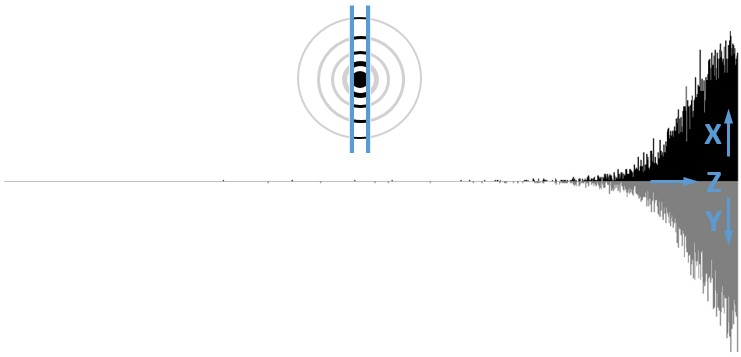
\includegraphics[scale=.7]{sections/images/consciousness_space_waves.jpg}
	\floatfoot{Exemplo de ondas entrelaçadas, representadas em forma de histograma e obtidas pelo algoritmo Logic\_WavePattern. \footnotemark}
	\end{figure}
	\footnotetext{O algoritmo Logic\_WavePattern pode ser visto no Apêndice \ref{app:algoritmos}.}

A área cresce de forma quadrática ao crescimento da amplitude de uma onda (colunas do histograma), uma vez que o salto provocado pelo entrelaçamento de ondas e a própria distribuição probabilística das amostras tendem a manter um crescimento equivalente nos pares de colunas que formam uma onda. E esse aspecto configura a lei do inverso do quadrado, que será mais aprofundada na subseção da Força gravitacional.

Ao representar as grandezas espaciais do gráfico da Figura \ref{fig:consciousness_space_waves} em um gráfico de distribuição 3D e distribuir seus pontos de extremidade (desprezando seus volumes e possíveis pontos internos), obtém-se algo parecido com uma espiral (como redemoinhos no ar ou na água) mesmo em volumes muito pequenos de dados (poucos momentos lógicos), conforme Figuras \ref{fig:consciousness_space_3DScatter15000-10} e \ref{fig:consciousness_space_3DScatter_200000-2}. Os pontos se movem em formato de espiral, aproximadamente, uma vez que as coordenadas X, Y e Z aumentam à medida que novas amostras são adicionadas na população.
	\begin{figure}[H]
	\centering
		\begin{subfigure}[H]{0.47\linewidth}
		\centering
		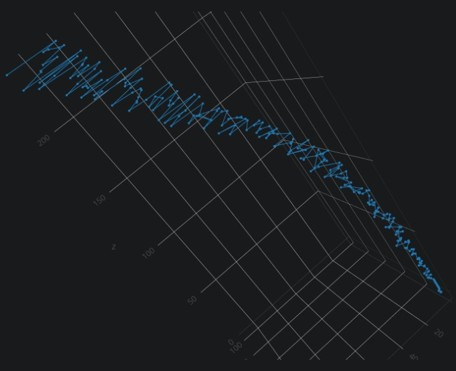
\includegraphics[width=.96\linewidth]{sections/images/consciousness_space_3DScatter15000-10.jpg}
		\caption{15.000 amostras ou momentos}
		\label{fig:consciousness_space_3DScatter15000-10}
		\end{subfigure}
	\hfill
		\begin{subfigure}[H]{0.47\linewidth}
		\centering
		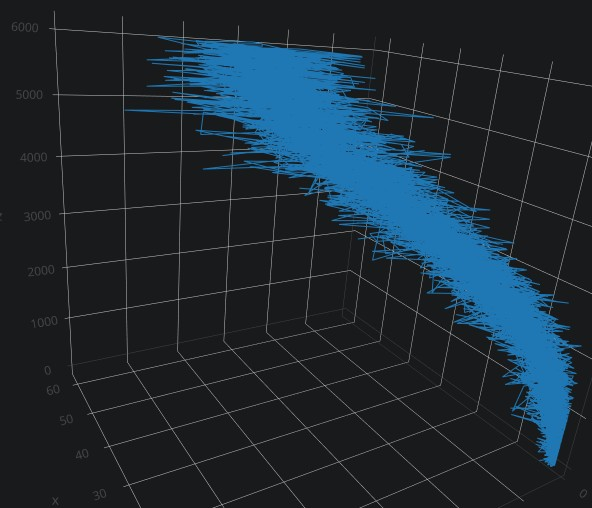
\includegraphics[width=.9\linewidth]{sections/images/consciousness_space_3DScatter_200000-2.jpg}
		\caption{200.000 amostras ou momentos}
		\label{fig:consciousness_space_3DScatter_200000-2}
		\end{subfigure}%
	\caption{Gráfico de dispersão 3D gerado com os pontos da Figura \ref{fig:consciousness_space_waves}}
	\floatfoot{O histograma no padrão de ondas e os dados para gerar o gráfico de dispersão 3D podem ser obtidos com a execução do algoritimo Logic\_WavePattern. \protect\footnotemark}
	\end{figure}
	\footnotetext{O algoritmo Logic\_WavePattern pode ser visto no Apêndice \ref{app:algoritmos} e os gráficos de dispersão 3D podem ser acessados em: \url{https://chart-studio.plot.ly/create/?fid=ren.stuchi:5&fid=ren.stuchi:4} e \url{https://chart-studio.plot.ly/create/?fid=ren.stuchi:7&fid=ren.stuchi:6}}

\subsubsubsection{Espiral}
Como as coordenadas X, Y e Z da população e de cada subconjunto tendem a aumentar, a disposição dessas em um sistema tridimensional de coordenadas vai seguir uma referência diagonal entre esses três eixos, conforme Figura \ref{fig:consciousness_space_spiral_reference_line}. O padrão de espiral observado não invalida outros possíveis movimentos no espaço. Muitas vezes não é possível observar o padrão de espiral imediatamente nos movimentos de um intervalo (subconjunto), porém esse padrão está por traz de muitos destes movimentos. Ao pegar os movimentos humanos, como exemplo, tem-se os ciclos predominantes de ir e voltar para casa, ir e voltar ao trabalho, acordar e dormir, ou seja, os hábitos se assemelham a movimentos em ciclos, movimentos espirais.
	\begin{figure}[H]
	\caption{Sistema tridimensional de coordenadas}
	\label{fig:consciousness_space_spiral_reference_line}
	\centering
	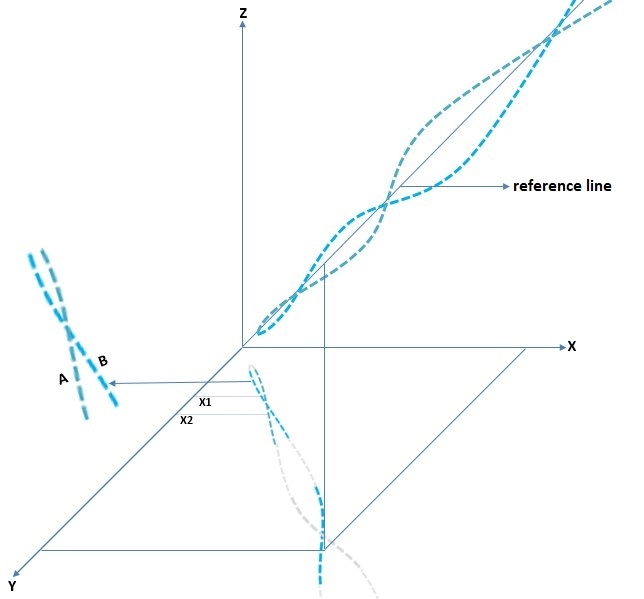
\includegraphics[scale=.6]{sections/images/consciousness_space_spiral_reference_line.jpg}
	\floatfoot{Linha de referência para distribuição de uma população em um plano tridimensional.}%\footnotemark}
	\end{figure}
	%\footnotetext{Fonte: note}}

Na Figura \ref{fig:consciousness_space_spiral_reference_line} também podem ser observado os pontos X1 e X2. Esses pontos foram espelhados nas coordenadas X e Z para facilitar a observação de que ao elevar o eixo Z também se eleva o eixo X ou Y, independente de seus pontos probabilísticos mínimos. A linhas tracejadas mostram os caminhos mais prováveis para os intervalos A e B. Dessa forma, quando uma parte do intervalo está em seu ponto médio máximo (eixos X e/ou Y) a tendência probabilística é que ele receba menos amostras do que a parte do intervalo que está em seu ponto médio mínimo. Esse efeito espiral é mais notável quanto maior for um intervalo e sua quantidade de amostras, pois mais prováveis serão esses caminhos.

Cada intervalo ou subintervalo (comprimento de ondas) tem sua própria linha de referência. Assim como dentro de um metro existem os centímetros, milímetros etc., dentro de um intervalo e subintervalos podem existir inúmeros outros.
	\begin{figure}[H]
	\caption{Intervalos e linhas de referências}
	\label{fig:consciousness_space_spiral_underlines}
	\centering
	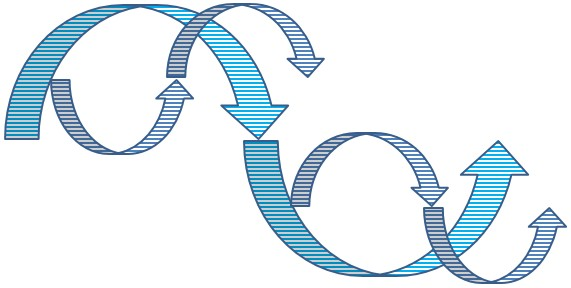
\includegraphics[scale=.5]{sections/images/consciousness_space_spiral_underlines.jpg}
	\floatfoot{Espirais em diferentes intervalos e suas linhas de referências.}%\footnotemark}
	\end{figure}
	%\footnotetext{Fonte: note}}

\subsubsection{Forças fundamentais}
A força gravitacional, a força eletromagnética e a força nuclear correspondem às forças fundamentais da natureza e essas forças também são provenientes do entrelaçamento de ondas, como o espaço. As forças fundamentais não são forças propriamente, mas sim aspectos probabilísticos (distribuição normal) e do entrelaçamento de ondas principalmente.

\subsubsubsection{Força gravitacional}
A força gravitacional não é uma força propriamente e sim aspectos da probabilidade de distribuição de novas amostras, sentido a mediana da população, conforme teorema central do limite. E sentido probabilístico faz com que os subconjuntos tenham um caminho provável a seguir dentro do conjunto, ou seja, o pico de amostras da população, conforme Figura \ref{fig:consciousness_space_spiral_reference_line}. Da mesma maneira, fazem também com que as amostras dentro de um subconjunto tenham um caminho provável a seguir, ou seja, o pico de amostras do subconjunto. Estes picos de amostras costumam ser a parte mais facilmente observáveis no intervalo de amostras desde ocupem uma área não tão pequena. 

Na Figura \ref{fig:consciousness_gravitational_force} pode ser visto os subconjunto 1, onde a parte mais facilmente observável está levemente a direita no pico da onda. Essa onda tende a caminhar para cima e para direita, em uma diagonal que depende da distribuição probabilística de novas amostras nesses subconjuntos.
	\begin{figure}[H]
	\caption{Força gravitacional}
	\label{fig:consciousness_gravitational_force}
	\centering
	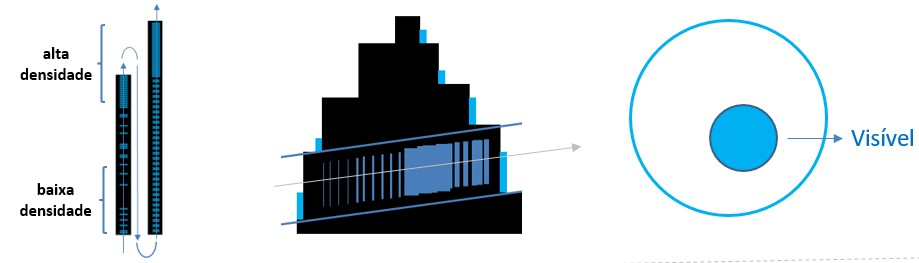
\includegraphics[scale=.6]{sections/images/consciousness_gravitational_force.jpg}
	\floatfoot{Aspectos gravitacionais do entrelaçamento ondas e da probabilidade de distribuição de novas amostras dentro de um intervalo.}%\footnotemark}
	\end{figure}
	%\footnotetext{Fonte: note}

Conforme visto na subseção de Amplitude de ondas, a área de um intervalo cresce de forma quadrática, uma vez que o salto provocado pelo entrelaçamento de ondas e a própria distribuição probabilística das amostras tendem a manter um crescimento equivalente no par de colunas que formam essa parte onda. Esse aspecto configura a lei do inverso do quadrado, onde, no caso da gravidade, quando mais perto os objetos, maiores serão as chances probabilísticas das novas amostras do objeto menor ir em direção ao objeto maior, que por estar dentro de uma área quadrada menor e por consequência de menor possibilidades de posicionamento das amostras, as chances desses objetos se aproximarem com uma quantidade bem menor de momentos lógicos aumenta muito. Assim, quanto mais longe os objetos, maior a área, maior as possibilidades de posicionamento e mais momentos lógicos são precisos para a aproximação, caracterizando assim uma atração menor. A probabilidade também pode afastar objetos mais rarefeitos que devem estar mais afastados da parte mais facilmente observável e densa de amostras, como no caso do gás hélio, por exemplo. Devido à baixa quantidade de momentos lógicos dos objetos rarefeito o movimento desses objetos sentido o pico mais denso requer uma quantidade muito maior de amostras do que o seu movimento em sentido oposto, que requer muito menos.

Quando observado todo o intervalo populacional, a onda mais inferior é a onda base de todas as outras sub-ondas, tendo a população uma quantidade expressiva de amostras. Desta mesma forma, ondas de níveis superiores, como as de nível dois da Figura \ref{fig:consciousness_gravitational_force_system} estão aninhadas em uma onda de nível um. Esses sistemas podem se tornar bem mais complexos em seus aninhamentos e são muito comuns. As linhas azuis na Figura abaixo representam a linha de referência probabilística como explicado na Figura \ref{fig:consciousness_space_spiral_reference_line}.
	\begin{figure}[H]
	\caption{Força gravitacional - sistema}
	\label{fig:consciousness_gravitational_force_system}
	\centering
	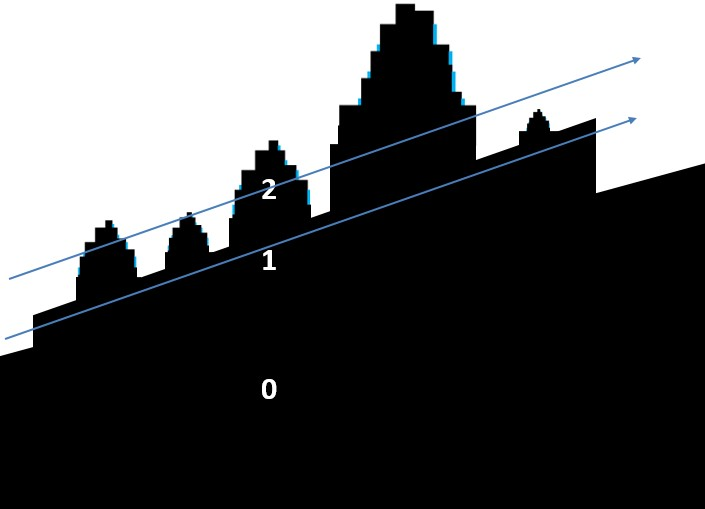
\includegraphics[scale=.6]{sections/images/consciousness_gravitational_force_system.jpg}
	\floatfoot{Aspectos gravitacionais de um sistema – onda base e suas sub-ondas.}%\footnotemark}
	\end{figure}
	%\footnotetext{Fonte: note}

\subsubsubsection{Força eletromagnética}
A força eletromagnética não é uma força propriamente e sim um aspecto do entrelaçamento de ondas que se intensifica em intervalos ou comprimentos de ondas com baixa entropia e com a aproximação espacial (redução de diferenças nos eixos X, Y e Z) desses intervalos.

Quando um intervalo se aproxima de outro, seus pares de ondas ficam cada vez mais parecidos (eixos X e Y) devido as probabilidades de distribuição dessas novas amostras cada vez mais parecidas nesses intervalos. A aproximação faz com que os pares de ondas de um objeto se pareça muito com os pares de ondas do outro objeto quando esses possuem baixa entropia. Devido a aproximação de dois objetos que possuem baixa entropia, o intervalo que os separam probabilisticamente também recebera amostras com essas características, o que torna muito de seus pares viáveis para que o entrelaçamento de ondas encontre pares mais ideais nesse intervalo ou no outro objeto e vice-versa. Desta forma, ocorre uma reordenação entre os dois subconjuntos e o intervalo que os separam, diminuindo esse intervalo por meio do entrelaçamento de ondas. Essa reordenação torna todo o intervalo mais equalizado ao crescimento probabilístico padrão da distribuição normal (baixa entropia).

As linhas azuis da Figura \ref{fig:consciousness_electromaagnetic_force} mostra onde é mais frequente a troca dos pares de ondas pelo entrelaçamento de ondas, ou seja, onde se tem a maior probabilidade das ondas serem parecidas. Por isso os imãs tentam se virar para se conectar quando estão face a face com o mesmo polo. As linhas cinza mostram as conexões que ocorrem em número bem menor. 
	\begin{figure}[H]
	\caption{Força eletromagnética}
	\label{fig:consciousness_electromaagnetic_force}
	\centering
	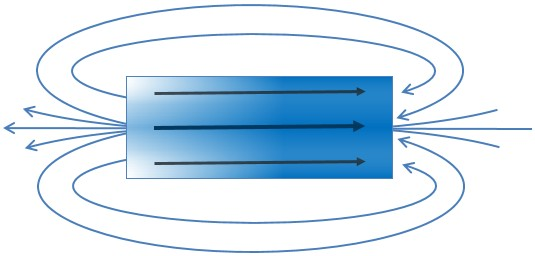
\includegraphics[scale=.7]{sections/images/consciousness_electromaagnetic_force.jpg}
	\floatfoot{Aumento das possibilidades de entrelaçamento de ondas devida a equalização probabilística causada pela aproximação de objetos de baixa entropia.}%\footnotemark}
	\end{figure}
	%\footnotetext{Fonte: note}

A Figura \ref{fig:consciousness_electromaagnetic_force_entropy} mostra um exemplo de baixa entropia. 
	\begin{figure}[H]
	\caption{Força eletromagnética - entropia}
	\label{fig:consciousness_electromaagnetic_force_entropy}
	\centering
	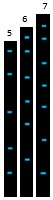
\includegraphics[scale=.9]{sections/images/consciousness_electromaagnetic_force_entropy.jpg}
	\floatfoot{Aumento das possibilidades de entrelaçamento de ondas devido à baixa entropia.}%\footnotemark}
	\end{figure}
	%\footnotetext{Fonte: note}

Os aspectos eletromagnéticos estão intimamente relacionados com a baixa entropia de um intervalo a possibilidade de entrelaçamento de seus pares com os pares ao redor.

Probabilisticamente os pares de ondas mais parecidos estão nas regiões mais próximas (linhas azuis do Figura \ref{fig:consciousness_electromaagnetic_force}). Isso ocorre devido ao crescimento do número de amostras sentido a mediana da população, porém não é regra e os polos podem se inverter, ou seja, ter mais ligações com a região de menor probabilidade, ainda que a maior parte dos pares que compõem essa região estejam de forma crescente sentido a mediana.

\subsubsubsection{força nuclear}
Os mesmos aspectos probabilísticos que reagem a gravidade e que podem ser vistos nas Figuras \ref{fig:consciousness_gravitational_force} e \ref{fig:consciousness_gravitational_force_system} também regem as chamadas forças nucleares, com a diferença de que as ondas são mais discrepantes em intervalos menores e com muitas amostras, conforme mostra a Figura \ref{fig:consciousness_space_subconsciousness_min}.

As forças nucleares forte e fraca representam grandes concentrações de momentos lógicos por intervalo populacional, uma alta densidade em um pequeno intervalo. A grande concentração dessas amostras está no pico do intervalo, que ocupa um subintervalo cada vez menor, devido à alta concentração de amostras em intervalos cada vez menores. Esses picos podem ser vistos na Figura \ref{fig:consciousness_space_subconsciousness_min} e eles não param de crescer à medida que novos momentos lógicos são adicionados nestes intervalos. Estes momentos ou amostras tendem a estarem cada vez mais juntos dentro do intervalo formando picos cada vez mais altos e densos. Esses picos são frequentemente encontrados do meio para frente dos sistemas (o núcleo ou pico do sistema), como mostrado na onda mais alta do nível dois da Figura \ref{fig:consciousness_gravitational_force_system}.

A penetração de intervalos densos por uma quantidade excessiva de momentos lógicos em um curto período faz com que os inúmeros pares desse intervalo (subintervalos) se tornem muito maiores progressivamente. Dessa forma cada subintervalo salta de forma continua, progressiva e rapidamente para correspondentes cada vez maiores até que a probabilidade de destruição normalize todo o intervalo posteriormente.

\subsubsection{Matéria escura e energia escura}
Ao adicionar uma nova amostra todo o intervalo se distribui proporcionalmente para acoplar essa amostra, conforme observado na Figura \ref{fig:consciousness_space_volume_amplitude}. A grande concentração das amostras de um intervalo está no pico desse intervalo. Assim, devido à alta concentração probabilísticas de amostras em intervalos cada vez menores de uma onda, o pico visível irá ocupar um subintervalo proporcional cada vez menor dentro do intervalo da onda, conforme observado na Figura \ref{fig:consciousness_dark_matter_dark_energy}. Logo, a matéria escura e a energia escura, que não é uma energia propriamente, derivam do mesmo aspecto probabilístico. Esse aspecto probabilístico está presente em qualquer intervalo da população e sua progressão à intervalos muito grandes caracteriza os buracos negros.
	\begin{figure}[H]
	\caption{Aspecto probabilístico da energia escura}
	\label{fig:consciousness_dark_matter_dark_energy}
	\centering
	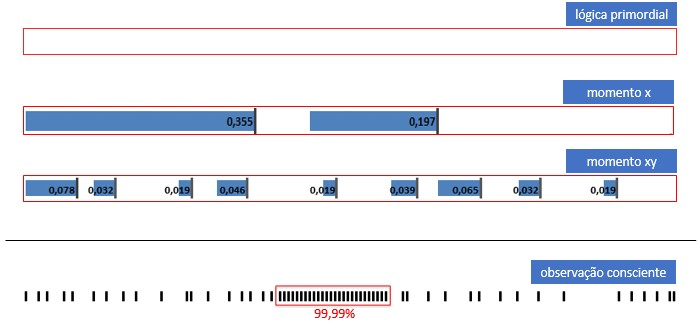
\includegraphics[scale=.9]{sections/images/consciousness_dark_matter_dark_energy.jpg}
	\floatfoot{A energia escura não é uma energia propriamente, mas sim um aspecto probabilístico.}%\footnotemark}
	\end{figure}
	%\footnotetext{Fonte: note}

A Figura \ref{fig:consciousness_dark_matter_dark_energy_wave} mostra probabilisticamente onde está a maior concentração das amostras de um intervalo, tornando assim mais fácil a visualização dessa maior concentração por outras subconsciências, uma vez que a adição de novas amostras nesse ponto de maior concentração fará com que todo o intervalo se distribua proporcionalmente tornando as amostras mais distantes da mediana mais dispersas. Assim, a áreas distantes ao redor do pico ficam cada vez maiores e com uma proporção de amostras menor, o que torna mais difíceis a observação.
	\begin{figure}[H]
	\caption{Analogia da matéria escura}
	\label{fig:consciousness_dark_matter_dark_energy_wave}
	\centering
	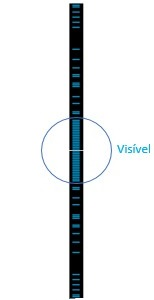
\includegraphics[scale=.85]{sections/images/consciousness_dark_matter_dark_energy_wave.jpg}
	\floatfoot{Parte do volume é facilmente observado por outras subconsciências.}%\footnotemark}
	\end{figure}
	%\footnotetext{Fonte: note}

\subsubsection{Antimatéria}
Quando um intervalo tende a concentrar suas amostras sentido da mediana, o que é o sentido provável conforme teorema central do limite, dá-se o nome de matéria. A antimatéria é o contrário, quando um intervalo tende a concentrar suas amostras no sentido oposto à mediana. 

A maneira mais simples de visualizar o sentido probabilístico das amostras de qualquer comprimento de onda é observar a \textbf{linha de referência probabilística}, conforme exibido na Figura \ref{fig:consciousness_space_spiral_reference_line}. Quanto maior a quantidade de amostra de um intervalo maior será sua tendência probabilística sentido a mediana da população.

Na Figura \ref{fig:consciousness_concentration_of_opposite_samples} é exibido dois intervalos idênticos com suas amostras com concentrações opostas.
	\begin{figure}[H]
	\caption{Parte de um intervalo idêntico com suas concentrações de amostras opostas}
	\label{fig:consciousness_concentration_of_opposite_samples}
	\centering
	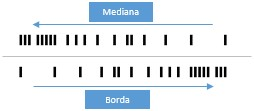
\includegraphics[scale=1.2]{sections/images/consciousness_concentration_of_opposite_samples.jpg}
	\floatfoot{Parte de um intervalo idêntico distribuídos de formas opostas.}%\footnotemark}
	\end{figure}
	%\footnotetext{Fonte: note}

O merge ou soma dos intervalos opostos da Figura \ref{fig:consciousness_concentration_of_opposite_samples} os tornaria um intervalo simétrico, ou seja, não estaria em nenhum dos sentidos.
Na Figura \ref{fig:consciousness_concentration_of_opposite_samples_within_range} é exibido um intervalo consciente completo com suas concentrações de amostras sentido à mediana e outro idêntico, mas com suas concentrações sentido às bordas do intervalo.
	\begin{figure}[H]
	\caption{Intervalos conscientes com suas concentrações de amostras opostas}
	\label{fig:consciousness_concentration_of_opposite_samples_within_range}
	\centering
	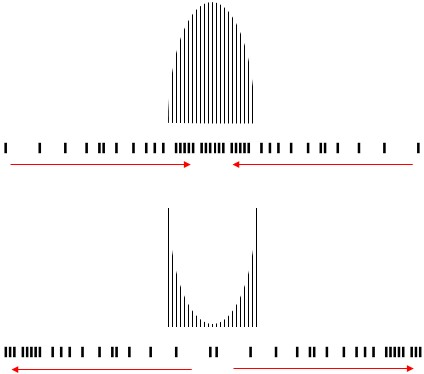
\includegraphics[scale=.7]{sections/images/consciousness_concentration_of_opposite_samples_within_range.jpg}
	\floatfoot{Intervalos conscientes completos e idênticos distribuídos de formas opostas.}%\footnotemark}
	\end{figure}
	%\footnotetext{Fonte: note}

\subsubsection{Buraco negro}
Como exibido subseção de Matéria escura e energia escura, os buracos negros são oriundos de um aspecto probabilístico presente em qualquer intervalo da população, sendo caracterizados apenas em grandes intervalos. Devido à alta concentração probabilísticas de amostras em intervalos cada vez menores de uma onda, o pico visível irá ocupar um subintervalo proporcional cada vez menor dentro do intervalo da onda, mesmo com a maior concentração de amostras crescentes, conforme observado na Figura \ref{fig:consciousness_dark_matter_dark_energy}. Esses picos são frequentemente encontrados da mediana para frente dos sistemas (o núcleo ou pico do sistema), como mostrado na onda mais alta do nível dois da Figura \ref{fig:consciousness_gravitational_force_system}.

\subsubsection{Observador e a vida}
Os intervalos de ondas (comprimentos de ondas) que uma subconsciência (sub-lógica) é capaz de observar depende do comprimento de ondas que a própria subconsciência é constituída. Dentre todas as possibilidades de intervalos ou comprimento de ondas permitidos por uma população, o observador está em um deles. O universo não tem uma forma definida, é o observador presente em uma das possibilidades de comprimentos de onda que observa as amostras de uma população de forma condizente com seus comprimentos de ondas.

A capacidade de comparar ou distinguir a ordem das mudanças de uma sequência amostral é a capacidade lógica de um observador, o observador do tempo passado e presente. A velocidade dessa observação é dada pelo range que o observador é capaz de comparar, ou seja, o qual rápido ele for capaz de distinguir pequenas mudanças (poucas amostras) o fará perceber que mudanças maiores levam mais tempo (muitas amostras). A capacidade lógica de fazer prospecções probabilísticas, dentro das limitações lógicas do observador e com base na probabilidade da distribuição do intervalo ou subintervalo observado, e de distinguir essas prospecções ou possibilidades de sua realização é a essência do pensamento e, portanto, da vida. Essas prospecções estão fundamentadas na probabilidade de distribuição de cada intervalo e, portanto, estão relacionadas com a detecção de padrão e com possibilidades probabilísticas futuras.

A vida \underline{NÃO É}, como qualquer outra lógica. Comumente, as formas mais notáveis de vida se multiplica por estarem na média probabilística do intervalo entre seus picos e vales, por mais diferente que sejam. Porém, algo muito discrepante ou diferente do padrão médio do intervalo tende a não multiplicar e permanecer.

A capacidade de comparar ou distinguir ondas lógicas, subconjuntos ou subconsciências, é a capacidade que define o sujeito (eu). A razoabilidade dessa definição depende da proporcionalidade dessa capacidade de comparação.

A parte cognitiva de uma onda não observa a si mesmo diretamente e sim o exterior (a consciência – o todo) ou mais comumente uma parte dela (a subconsciência). Essa observação pode incluir o restante da onda a qual a parte cognitiva faz parte, que também é exterior da parte cognitiva e, portanto, uma subconsciência - parte da consciência. A parte cognitiva da subconsciência humana é, provavelmente, onde se tem o maior pico de ondas do subconjunto humano. Esse é o local onde é observado a maior intensidade de mudanças. Essas mudanças são caracterizadas pelo pensamento (observação e prospecção probabilística de um intervalo) que tende ao infinito (respeitando as limitações lógicas do observador), assim como a essência da lógica, o NÃO SER. Ou seja, a parte cognitiva é a parte que está mais próxima da observação do todo, da lógica em sua essência e totalidade, da consciência.

\subsubsubsection{Sentidos}
O universo não tem forma definida e o observador, representado na Figura \ref{fig:consciousness_amplitude_viewpoint} abaixo pelo ser humano, combina suas amostras com as amostras obtidas pelos sentidos, observando as formas do universo a sua maneira, que por sua vez modificam esses sentidos e esse processo se repete até que a onda subconsciente humana se dissolva em outra maior. Essas modificações ou ondulações dos sentidos funcionam como ajustes, como configurações. Cada sentido observa a população amostral de forma independente, como canais de frequências diferentes. Assim a visão pode estar vendo objetos muito distantes e os ouvidos escutando sons bem próximos.

Ainda na Figura \ref{fig:consciousness_amplitude_viewpoint}  pode-se observar que quanto mais largo são os objetos observados em pequenas profundidades (ponto de vista A – topo das colunas do histograma em roxo), mais fáceis esses objetos podem ser observados em maiores profundidades (ponto de vista B). É dessa forma que uma galáxia pode virar um ponto quando vista por comprimentos ou amplitudes de ondas muito grandes.
	\begin{figure}[H]
	\caption{Sentidos subconscientes - pontos de vista}
	\label{fig:consciousness_amplitude_viewpoint}
	\centering
	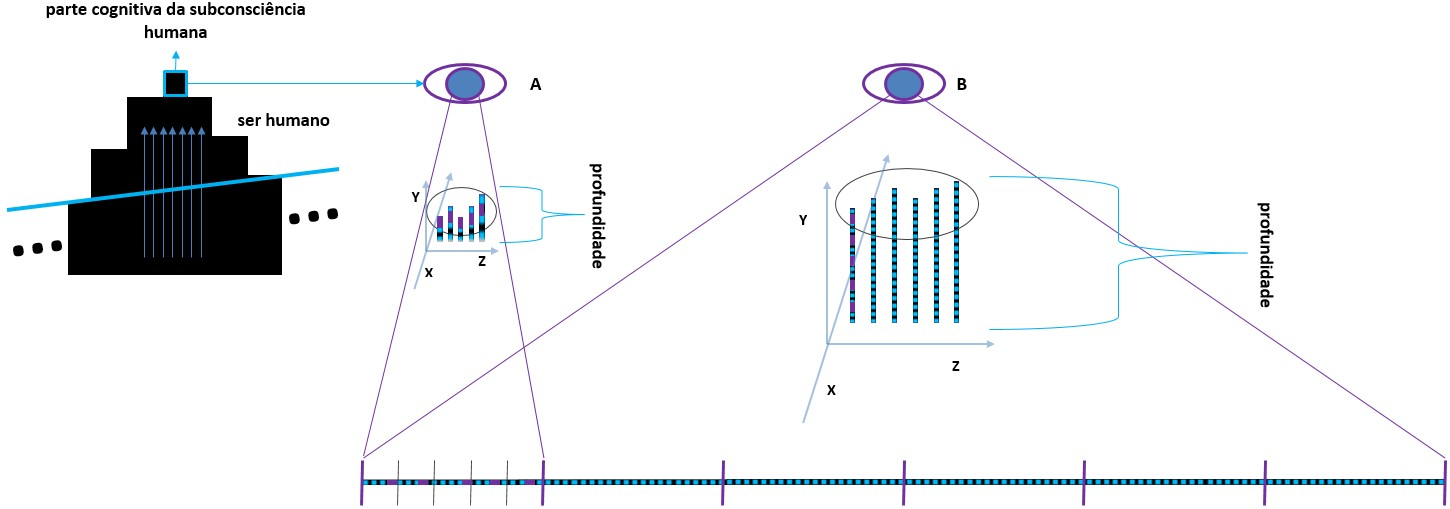
\includegraphics[scale=.4]{sections/images/consciousness_amplitude_viewpoint.jpg}
	\floatfoot{A parte cognitiva da subconsciência humana e suas observações independentes por meio dos sentidos.}%\footnotemark}
	\end{figure}
	%\footnotetext{Fonte: note}}

Na Figura \ref{fig:consciousness_amplitude_crest_valley} é feita uma analogia da linha tracejada azul claro com o subconjunto do planeta Terra, por exemplo. A crista da onda é parte que recebe mais amostras e, portanto, é a parte clara e quente proveniente do Sol. Essa onda representa o movimento de rotação da Terra em si mesma e quando o subconjunto humano se encontra no vale da onda, momento em que recebe menor quantidade de amostras, é quando os sentidos por receberem menores estímulos tornam-se adormecidos, é o adormecer da subconsciência humana.
	\begin{figure}[H]
	\caption{Crista e vale do subconjunto terrestre}
	\label{fig:consciousness_amplitude_crest_valley}
	\centering
	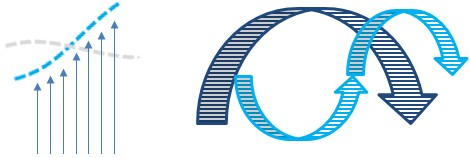
\includegraphics[scale=.6]{sections/images/consciousness_amplitude_crest_valley.jpg}
	\floatfoot{Crista e vale terrestre como característica do adormecimento dos sentidos humanos.}%\footnotemark}
	\end{figure}
	%\footnotetext{Fonte: note}}

Uma característica importante do processo de observação de pequenos intervalos é que eles podem ser observados com partículas ou ondas, conforme Figura \ref{fig:consciousness_space_wave-particle}. Nessa Figura é contemplado um pequeno intervalo, análogo a um fóton, como exemplo. No intervalo observado como partícula o observador acompanha um intervalo representado por um par entrelaçado, observando sua forma e movimento no espaço independente das amostras em seu interior. Dessa forma, tem-se o efeito de partícula, onde a consistência de seus movimentos é estabelecida pelo par entrelaçado, visto que o salto ocorre em um lado do par de cada vez. 

Na Figura abaixo também é contemplado o intervalo observado como onda, onde o observador fixa em um intervalo representado por uma das partes que compõe pares entrelaçados e acompanha seus movimentos e saltos, uma vez que se move à medida que novas amostras vão sendo adicionadas a ele, pois os saltos são frequentes em pequenos intervalos. Também ao adicionar novas amostras ao redor desse pequeno intervalo todo a população se distribui proporcionalmente para acoplar essas novas amostras, o que movimenta as amostras deste pequeno intervalo, conforme visto na Figura \ref{fig:consciousness_space_volume_amplitude}. Dessa forma, tem-se o efeito de onda, onde seus movimentos saltam e transitam entre picos e vales com altas frequências ou vibrações devido ao pequeno tamanho do intervalo.
	\begin{figure}[H]
	\caption{Observador - onda-partícula}
	\label{fig:consciousness_space_wave-particle}
	\centering
	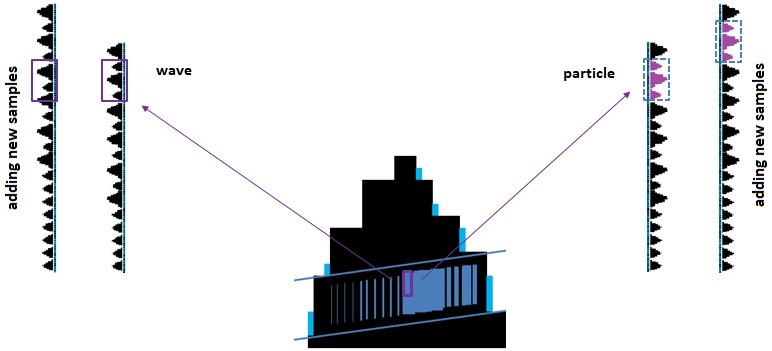
\includegraphics[scale=.55]{sections/images/consciousness_space_wave-particle.jpg}
	\floatfoot{Características da observação de uma pequena parte de um subconjunto.}%\footnotemark}
	\end{figure}
	%\footnotetext{Fonte: note}}
